\documentclass[12pt]{article}

\usepackage[T1]{fontenc}
\usepackage[utf8]{inputenc}
\usepackage{lmodern}
\usepackage{amsthm}
\usepackage{amssymb}
\usepackage{amstext}
\usepackage{bm}
\usepackage{graphicx}
\usepackage{epstopdf}
\usepackage{subcaption}
\usepackage[breaklinks=true]{hyperref}
\usepackage{amsmath}
\usepackage{setspace}
\usepackage[capitalize]{cleveref}

% cleveref package
\crefalias{subequation}{equation}
\crefformat{pluraleq}{Eqs.~(#2#1#3)}

\pagestyle{plain}
% Margins
\renewcommand{\baselinestretch}{1.0} 
\setlength{\topmargin}{-0.5in} 
\setlength{\oddsidemargin}{0.25in} 
\setlength{\evensidemargin}{0.25in} 
\setlength{\textwidth}{6.0in} 
\setlength{\textheight}{9.0in} 
\setlength{\parskip}{0pt}    

% Labels of tables, sections, equations
\renewcommand\thetable{\Roman{table}}
\renewcommand{\thesection}{\Roman{section}} 
\renewcommand{\thesubsection}{\thesection.\Alph{subsection}}
\renewcommand{\theequation}{\arabic{equation}}

% hyperlinks
\hypersetup{colorlinks=true,
  pdftitle={Nonclassical Particle Transport in 1-D Random Periodic Media},
  pdfauthor={Richard Vasques and Kai Krycki and Rachel Slaybaugh}
}

\newcommand{\bl}{\big<}
\newcommand{\bg}{\big>}
\newcommand{\R}{\mathbb{R}}
\newcommand{\eps}{\varepsilon}
\renewcommand{\vec}[1]{\mathbf{#1}}
\newcommand{\mat}[1]{\mathbf{#1}}
\newcommand{\ux}{{\bm x}}
\newcommand{\un}{{\bf n}}
\newcommand{\uomega}{{\bf \Omega}}
\newcommand{\unabla}{{\bf \nabla}}
\newcommand{\ul}{\underline}
 \newcommand{\Keywords}[1]{\vspace{12pt}\par\noindent
{\small{\bf Keywords\/}: #1}}




\begin{document}

\title{Nonclassical Particle Transport in 1-D Random Periodic Media}
\author{{\bf Richard Vasques}\footnote{Email: \texttt{richard.vasques@fulbrightmail.org}}\\
\em University of California, Berkeley\\
\em Department of Nuclear Engineering\\
\em 4103 Etcheverry Hall\\
\em Berkeley, CA 94720-1730 \\
\and {\bf Kai Krycki} \\
\em Aachen Institute for Nuclear Training GmbH \\
\em Jesuitenstraße 4, 52062 Aachen, Germany\\
\and {\bf R.\ N.\ Slaybaugh}\\
\em University of California, Berkeley\\
\em Department of Nuclear Engineering\\
\em 4173 Etcheverry Hall\\
\em Berkeley, CA 94720-1730}
\date{}
\maketitle

\begin{abstract}

TO BE WRITTEN

\Keywords{TBD}
\end{abstract}

\pagebreak

\doublespacing

\section{Introduction}

The classical theory of linear particle transport defines the total cross section $\Sigma_t$ as independent of the path-length $s$ (the distance traveled by the particle since its previous interaction) and of the direction of flight $\uomega$.
This definition leads to an exponential probability density function for a particle's distance-to-collision:
\begin{align}\label{eq1}
p(s) = \Sigma_t e^{-\Sigma_t s}.
\end{align}

However, a nonexponential attenuation law for the particle flux arises in certain inhomogeneous media in which the scattering centers are spatially correlated.
This ``nonclassical" behavior occurs in certain important applications, such as neutron transport in Pebble Bed Reactors (in which a nonexponential $p(s)$ arises due to the pebble arrangement within the core) and photon transport in atmospheric clouds (in which the locations of the water droplets in the cloud seem to be correlated in ways that measurably affect the radiative transfer within the cloud).

An approach to this type of nonclassical transport problem was recently proposed \cite{lar07,larvas11}, with the assumption that the positions of the scattering
centers are correlated but independent of direction $\uomega$.
Existence and uniqueness of solutions are rigorously discussed in \cite{fra10}.
This nonclassical theory was extended in \cite{vaslar14a} to include angular-dependent path-length distributions in order to investigate anisotropic diffusion of neutrons in 3-D PBR cores.

A similar kinetic equation with path-length as an independent variable has been rigorously derived for the periodic Lorentz gas in a series of papers by Golse et al.~(cf.~\cite{gol12} for a review), and by Marklof \& Str\"ombergsson (cf.~\cite{mar11,mar15}).
Furthermore, related work has been performed by Grosjean in \cite{gro51}; it considers a generalization of neutron transport that includes arbitrary path-length distributions, and presents a derivation of diffusion solutions for infinite isotropic point and plane source problems.
 
Assuming monoenergetic transport and isotropic scattering, the nonclassical linear Boltzmann equation with angular-dependent path-length distributions and isotropic source is writen as
\begin{align}\label{eq2}
\frac{\partial\psi}{\partial s}(\ux,\uomega,s) + &\uomega\cdot\unabla \psi(\ux,\uomega,s) + \Sigma_t(\uomega,s)\psi(\ux,\uomega,s) 
\\&= \frac{\delta(s)}{4\pi}\left[ c\int_{4\pi}\int_0^\infty \Sigma_t(\uomega',s')\psi(\ux,\uomega',s')ds' d\Omega' + Q(\ux) \right]\,, \nonumber
\end{align}
where $\ux = (x,y,z)=$ position, $\uomega = (\Omega_x,\Omega_y,\Omega_z)=$ direction of flight (with $|\uomega|=1$), $\psi$ is the nonclassical angular flux, $c$ is the scattering ratio (such that the scattering cross section $\Sigma_s= c\Sigma_t$), and $Q$ is the source.
Here, the nonclassical angular-dependent ensemble-averaged total cross section $\Sigma_t(\uomega,s)$
is defined as
\begin{align}\label{eq3}
\Sigma_t(\uomega,s)ds =  \begin{array}{l}
\text{ the probability (ensemble-averaged over all physical}\vspace{-10pt}\\
\text{ realizations) that a particle, scattered or born at any}\vspace{-10pt}\\
\text{ point $\ux$ and traveling in the direction $\uomega$, will experience}\vspace{-10pt}\\
\text{ a collision between $\ux + s\uomega$ and $\ux + (s+ds)\uomega$.}
\end{array}
 \end{align}
The underlying path-length distribution and the above nonclassical cross section are related \cite{vaslar14a} by
\begin{align}\label{eq4}
	p(\uomega,s) = \Sigma_t(\uomega,s)\exp\left( -\int_0^s\Sigma_t(\uomega,s')ds'\right).
\end{align}
It has been shown that, if $p(s)$ is independent of $\uomega$, \cref{eq2} can be converted to an integral equation for the scalar flux that is identical to the integral equation that can be constructed for certain diffusion-based approximations \cite{siap15,vas16}.

Moreover, if the path-length distribution function is an exponential as given in \cref{eq1}, \cref{eq2} reduces to the classical linear Boltzmann equation
\begin{subequations}\label[pluraleq]{eq5}
\begin{align}\label{eq5a}
\uomega\cdot{\unabla} \Psi(\ux,\uomega) + \Sigma_t\Psi(\ux,\uomega) = \frac{1}{4\pi}\left[\int_{4\pi}\Sigma_s\Psi(\ux,\uomega')d\Omega' + Q(\ux) \right]\,
\end{align}
for the classical angular flux 
\begin{align}
\Psi(\ux,\uomega) = \int_0^\infty \psi(\ux,\uomega,s)ds.
\end{align} 
\end{subequations}

Numerical results have been provided for the asymptotic diffusion limit of this nonclassical theory \cite{larvas11,vaslar09,vas13,vaslar14b}, and for moment models of the nonclassical equation in the diffusive regime \cite{kry13}.
However, very few results have been presented for the nonclassical \textit{transport} equation.
This is because one must know $\Sigma_t(\uomega,s)$, or $\Sigma_t(s)$ in the case of angular-independent path lengths, in order to solve \cref{eq2}. 

In this paper, we present a numerical investigation of the accuracy of the nonclassical transport equation.
We consider a 1-D random periodic system: a spatially periodic system consisting of alternating layers, randomly placed on the $x-$axis.
This means that we only know which material is present at any given point $x$ in a probabilistic sense.
The 1-D version of \cref{eq2} is written as
\begin{align}\label{eq6}
\frac{\partial\psi}{\partial s}(x,\mu,s) + \mu\frac{\partial \psi}{\partial x}(x,\mu,s) &+ \Sigma_t(\mu,s)\psi(x,\mu,s) 
\\& = \frac{\delta(s)}{2}\left[ c\int_{-1}^1\int_0^\infty \Sigma_t(\mu',s')\psi(x,\mu',s')ds' d\mu' + Q(x) \right]\,. \nonumber
\end{align}
This system was chosen because we can obtain an analytical expression for the distribution function $p(\mu,s)$ of a particle's distance-to-collision in the direction $\mu$.
Then, using the identity \cite{vaslar14a}
\begin{align}\label{eq7}
\Sigma_t(\mu,s)=\frac{p(\mu,s)}{1-\int_0^sp(\mu,s')ds'},
\end{align}
we can obtain a solution for \cref{eq6}.

MORE TO COME

The remainder of this paper is organized as follows...    

\section{The 1-D Random Periodic System}\label{sec2}

Let us consider a 1-D physical system similar to the one introduced in \cite{zuc94}, consisting of alternating layers of two distinct materials (labeled 1 and 2) periodically arranged.
The period is given by $\ell = \ell_1 + \ell_2$, where $\ell_i$ represents the length of each layer of material $i \in \{1,2\}$.
A sketch of the periodic system is given in \cref{fig1}.
\begin{figure}[htb]
  \centering
  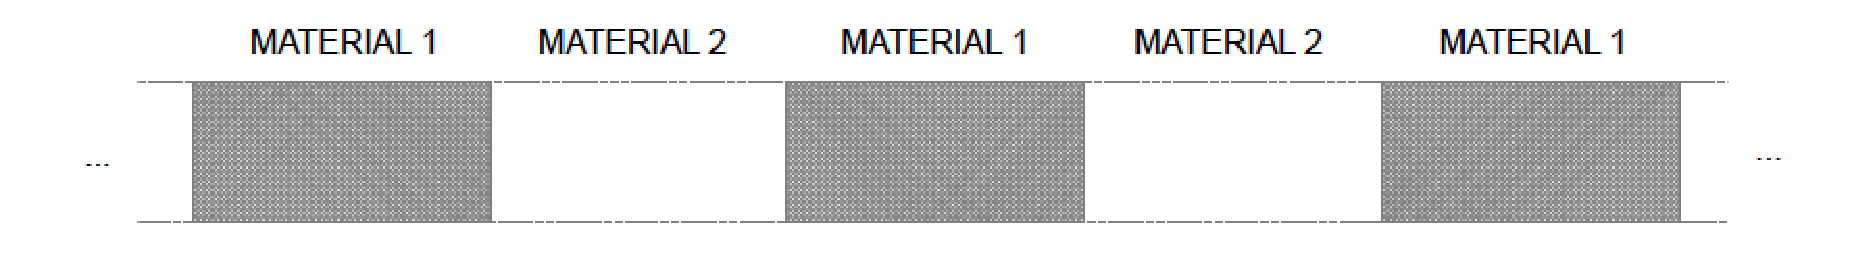
\includegraphics[width=\textwidth]{fig1.eps}
  \caption{A sketch of the periodic medium}
  \label{fig1}
\end{figure}

This periodic system is {\em randomly placed} in the infinite line $-\infty < x < \infty$, such that the probability $P_i$ of finding material $i$ in a given point $x$ is $\ell_i/\ell$.
Therefore, the cross sections and source are stochastic functions of space; that is, if $x$ is in material $i$, then
\begin{subequations}\label[pluraleq]{eq8}
\begin{align}
\Sigma_t(x) &= \Sigma_{ti}\, ,\\
\Sigma_s(x) &= c_i \Sigma_{ti}\, ,\\
Q(x) &= Q_i(x) \, ,
\end{align}
\end{subequations}
where $\Sigma_{ti}$, $c_i$, and $Q_i$ represent the total cross section, scattering ratio, and source in material $i$. 

\section{The Path-length Distribution Function}\label{sec3}

Given a physical realization of the 1-D system described in \cref{sec2}, let us examine a particle that is born (or scatters) at a point $x$ in a layer of material $i \in \{1,2\}$ with direction of flight $\mu\neq 0$.
We define $x_0$ to be the horizontal distance between $x$ (the point in which the collision or birth event took place) and the next intersection between layers in the direction $\mu$.
We also define:
\begin{subequations}\label[pluraleq]{eq9}
\begin{align}
p_{A_i}(x_0,\mu,s) &= \begin{array}{l}
\text{ the probability that a particle born or scattered in}\vspace{-10pt}\\
\text{ material $i$, at a horizontal distance $x_0$ of the next}\vspace{-10pt}\\
\text{ intersection, with direction of flight $\mu$, will travel a}\vspace{-10pt}\\
\text{ distance $s$ without colliding;}
\end{array}
\\
p_{B_i}(x_0,\mu,s)ds &= \begin{array}{l}
\text{ the probability that a particle born or scattered in}\vspace{-10pt}\\
\text{ material $i$, at a horizontal distance $x_0$ of the next}\vspace{-10pt}\\
\text{ intersection, with direction of flight $\mu$, will experience}\vspace{-10pt}\\
\text{  a collision between $s$ and $s+ds$.}
\end{array}
\end{align}
\end{subequations}
For $\mu\neq 0$, we can write
\begin{subequations}\label[pluraleq]{eq10}
\begin{align}
p_{A_i}(x_0,\mu,s) &=  \left\{
\begin{array}{ll}
e^{-\Sigma_{ti}s}, & \text{if } 0\leq s|\mu|\leq x_0\\
(e^{-\Sigma_{ti}x_0/|\mu|})(e^{-\Sigma_{tj}(s-x_0/|\mu|)}), &\text{if } x_0< s|\mu|\leq x_0+\ell_j\\
(e^{-\Sigma_{ti}(s-\ell_j/|\mu|)})(e^{-\Sigma_{tj}\ell_j/|\mu|}), &\text{if } x_0+\ell_j< s|\mu|\leq x_0+\ell\\
\,\,\,\vdots & 
\end{array}
\right.
\end{align}
and
\begin{align}
p_{B_i}(x_0,\mu,s) &=  \left\{
\begin{array}{ll}
\Sigma_{ti}, & \text{if } 0\leq s|\mu|\leq x_0\\
\Sigma_{tj}, &\text{if } x_0< s|\mu|\leq x_0+\ell_j\\
\Sigma_{ti}, &\text{if } x_0+\ell_j< s|\mu|\leq x_0+\ell\\
\,\,\,\vdots & 
\end{array}
\right.
\,\,,
\end{align}
\end{subequations}
such that
\begin{subequations}\label[pluraleq]{eq11}
\begin{align}
p_{A_i}(x_0,\mu,s) &=  \left\{
\begin{array}{ll}
e^{-\Sigma_{ti}s}, & \text{if } 0\leq s|\mu|\leq x_0  \\
e^{-\Sigma_{tj}s-(\Sigma_{ti}-\Sigma_{tj})(x_0+n\ell_i)/|\mu|}, & \text{if } x_0+n\ell< s|\mu|\leq  x_0+n\ell+\ell_j \\
e^{-\Sigma_{ti}s-(\Sigma_{tj}-\Sigma_{ti})(n+1)\ell_j/|\mu|}, & \text{if } x_0+n\ell+\ell_j< s|\mu|\leq x_0+(n+1)\ell
\end{array}
\right.
\end{align}
and
\begin{align}
p_{B_i}(x_0,\mu,s) &=  \left\{
\begin{array}{ll}
\Sigma_{ti}, & \text{if } 0\leq s|\mu|\leq x_0\\
\Sigma_{tj}, &\text{if } x_0+n\ell< s|\mu|\leq  x_0+n\ell+\ell_j\\
\Sigma_{ti}, &\text{if } x_0+n\ell+\ell_j< s|\mu|\leq x_0+(n+1)\ell
\end{array}
\right.
\,\,.
\end{align}
\end{subequations}
Here, $n=0, 1, 2, ...$; $i,j \in\{1,2\}$; $i\neq j$; and $\ell = \ell_i+\ell_j$. It is clear that
\begin{align}\label{eq12}
p_{C_i}(x_0,\mu,s)ds &= \begin{array}{l}
\text{ the probability that a particle born or scattered in}\vspace{-10pt}\\
\text{ material $i$, at a horizontal distance $x_0$ of the next}\vspace{-10pt}\\
\text{ intersection, with direction of flight $\mu$, will experience}\vspace{-10pt}\\
\text{ its \textit{first collision} while traveling a distance between $s$}\vspace{-10pt}\\
\text{  and $s+ds$}
\end{array}
\\&= \,\,\,p_{A_i}(x_0,\mu,s)\times p_{B_i}(x_0,\mu,s)ds, \nonumber
\end{align}
and the \textit{ensemble-averaged} path-length distribution function of particles born or scattered in material $i$ with direction of flight $\mu$ is given by
\begin{align}\label{eq13}
p_i(\mu,s) &= \frac{1}{\ell_i}\int_0^{\ell_i} p_{C_i}(x_0,\mu,s) dx_0.
\end{align}
Finally, the ensemble-averaged path-length distribution function for particles born {\em anywhere} in the 1-D random periodic system with direction of flight $\mu$ is given by the weighted average
\begin{align}\label{eq14}
p(\mu,s) &= \lambda_1 p_1(\mu,s) + \lambda_2p_2(\mu,s),
\end{align}
where $\lambda_i$ is the probability that any given birth or scattering event takes place in material $i$.
It is easy to see that if $\Sigma_{t1}=\Sigma_{t2}$, \cref{eq11} to \labelcref{eq14} yield the exponential
\begin{align}\label{eq15}
p(\mu,s)=p(s)=\Sigma_{t1}e^{-\Sigma_{t1}s},
\end{align}
as given in \cref{eq1}. 

\subsection{Solid-Void Medium}
\label{sec3A}

The numerical results included in this paper are for solid-void systems.
We define material 2 as the void, such that $\lambda_2=\Sigma_{t2}=Q_2=0$, $\lambda_1=1$, and $p(\mu,s) = p_1(\mu,s)$.
Depending on the lengths $\ell_i$ of the material layers, \cref{eq13} yields the following expressions for $p(\mu,s)$:
\begin{subequations}\label[pluraleq]{eq16}
\begin{itemize}
\item Case 1: $\ell_1<\ell_2$
\end{itemize}
\begin{align}
p(\mu,s) = \left\{
\begin{array}{ll}
\frac{\Sigma_{t1}}{\ell_1}(n\ell +\ell_1-s|\mu|)e^{-\Sigma_{t1}(s-n\ell_2/|\mu|)}, & \text{if } n\ell\leq s|\mu| \leq n\ell+\ell_1\\
0, & \text{if } n\ell+\ell_1 \leq s|\mu| \leq n\ell+\ell_2\\
\frac{\Sigma_{t1}}{\ell_1}(s|\mu|-n\ell-\ell_2)e^{-\Sigma_{t1}[s-(n+1)\ell_2/|\mu|]}, & \text{if } n\ell+\ell_2 \leq s|\mu| \leq (n+1)\ell\\
\end{array}
\right.
\end{align}
\begin{itemize}
\item Case 2: $\ell_1=\ell_2$
\end{itemize}
\begin{align}
p(\mu,s) = \left\{
\begin{array}{ll}
\frac{\Sigma_{t1}}{\ell_1}(n\ell +\ell_1-s|\mu|)e^{-\Sigma_{t1}(s-n\ell_2/|\mu|)}, & \text{if } n\ell\leq s|\mu| \leq n\ell+\ell_1\\
\frac{\Sigma_{t1}}{\ell_1}(s|\mu|-n\ell-\ell_2)e^{-\Sigma_{t1}[s-(n+1)\ell_2/|\mu|]}, & \text{if } n\ell+\ell_2 \leq s|\mu| \leq (n+1)\ell\\
\end{array}
\right.
\end{align}
\begin{itemize}
\item Case 3: $\ell_1>\ell_2$
\end{itemize}
\begin{align}
p(\mu,s) = \left\{
\begin{array}{ll}
\frac{\Sigma_{t1}}{\ell_1}(n\ell +\ell_1-s|\mu|)e^{-\Sigma_{t1}(s-n\ell_2/|\mu|)}, & \\
\hspace{6cm}\text{if } n\ell\leq s|\mu| \leq n\ell+\ell_2 & \\
\frac{\Sigma_{t1}}{\ell_1}[(n\ell +\ell_2-s|\mu|)(1-e^{\Sigma_{t1}\ell_2/|\mu|}) +\ell_1-\ell_2]e^{-\Sigma_{t1}(s-n\ell_2/|\mu|)}, & \\
\hspace{6cm}\text{if } n\ell+\ell_2\leq s|\mu| \leq n\ell+\ell_1 & \\
\frac{\Sigma_{t1}}{\ell_1}(s|\mu|-n\ell-\ell_2)e^{-\Sigma_{t1}[s-(n+1)\ell_2/|\mu|]}, & \\
\hspace{6cm}\text{if } n\ell+\ell_1 \leq s|\mu| \leq (n+1)\ell & 
\end{array}
\right.
\end{align}
\end{subequations}
where $n=0, 1, 2, ...$ .
Assuming $\Sigma_{t1}=1$ and direction of flight $\mu=\pm 1$, \cref{fig2} depicts the comparisons between numerically obtained (through Monte Carlo) path-length distributions and the analytical expressions given in \cref{eq16}. 
% We may want to indicate the Monte Carlo code. Perhaps as a footnote state that this is
%  currently an inhouse code but one that is being added to pyne and will therefore be 
% available in an open source way soon. One of the things I care a lot about is reproducibility.
% It would be cool to have the final version of this paper point to the functions in pyne and 
% then host the input, output, and scripts for making the plots somewhere like figshare. We can
% then site the DOI of everything needed to independently reproduce the results :)
\begin{figure}[hbt]
    \centering
    \begin{subfigure}{0.495\textwidth}
        \centering
        \includegraphics[width=\textwidth]{fig2a.eps}
        \caption{Case 1: $\ell_1=0.5$, $\ell_2=1.0$}
        \label{fig2a}
    \end{subfigure}
    \hfill
    \begin{subfigure}{0.495\textwidth}
        \centering
        \includegraphics[width=\textwidth]{fig2b.eps}
        \caption{Case 2: $\ell_1=\ell_2=1.0$}
        \label{fig2b}
    \end{subfigure}
    \\
    \begin{subfigure}{0.495\textwidth}
        \centering
        \includegraphics[width=\textwidth]{fig2c.eps}
        \caption{Case 3: $\ell_1=1.0$, $\ell_2=0.5$}
        \label{fig2c}
    \end{subfigure}
    \caption{Examples of path-length distribution functions in the directions $\mu=\pm 1$ in a solid-void 1-D random periodic medium with $\Sigma_{t1}=1.0$ }
    \label{fig2}
\end{figure}

TO BE WRITTEN: FIRST AND SECOND MOMENTS $\bl s \bg$ and $\bl s^2\bg$.

\section{Test Problems and Models}\label{sec4}

The test problems simulated in this paper consider only {\em rod geometry} transport (particles can only travel in the directions $\mu = \pm1$) taking place in a finite 1-D random periodic system with vacuum boundaries.
The classical transport equation with these restrictions is written as
\begin{subequations}\label[pluraleq]{eq17}
\begin{align}
&\pm \frac{\partial \Psi^{\pm}}{\partial x}(x) + \Sigma_t(x)\Psi^{\pm}(x) 
= \frac{\Sigma_s(x)}{2}\left[\Psi^{+}(x)+\Psi^{-}(x)\right]+ \frac{Q(x)}{2}\,,
\,\,\,-X\leq x\leq X,\\
&\Psi^+(-X) = \Psi^-(X) = 0\,,
\end{align}
\end{subequations}
where $\Psi^{\pm}(x) = \Psi(x,\mu=\pm 1)$ and the stochastic parameters $\Sigma_t(x)$, $\Sigma_s(x)$, and $Q(x)$ are given by \cref{eq8}.

We are interested in how accurately the nonclassical model predicts the ensemble-averaged scalar flux $\bl\Phi\bg$ (over all physical realizations).
To this end, we compare the nonclassical results against ``benchmark" results obtained by averaging the solutions of the transport equation over a large number of physical realizations of the random system.
Finally, we compare the performance of the nonclassical model against the widely-known atomic mix model.
\begin{table}[htb]
\centering
\caption{\bf Parameters of test problems}
\label{tab1} 
\begin{tabular}{||c|c|c|c|c||} \hline \hline
\textbf{Set}  & $\ell_1$ & $\ell_2$ & $\Sigma_{t1}$ &$c_1$ \\ \hline\hline
\textbf{A} & 0.5 & 1.0 & 1.0 & 0; 0.1; 0.2; 0.3; 0.4; 0.5; 0.6; 0.7; 0.8; 0.9; 0.95; 0.99\\
\hline
\textbf{B} & 1.0 & 1.0 & 1.0 & 0; 0.1; 0.2; 0.3; 0.4; 0.5; 0.6; 0.7; 0.8; 0.9; 0.95; 0.99\\
\hline
\textbf{C} & 1.0 & 0.5 & 1.0 & 0; 0.1; 0.2; 0.3; 0.4; 0.5; 0.6; 0.7; 0.8; 0.9; 0.95; 0.99\\
\hline
\textbf{D} & ??? & ??? & ??? & 0; 0.1; 0.2; 0.3; 0.4; 0.5; 0.6; 0.7; 0.8; 0.9; 0.95; 0.99\\
 \hline\hline  
  \end{tabular}
\end{table}


We consider a total of 48 problems divided in 4 sets, with vacuum boundaries at $\pm X=\pm 10$, and parameters given in \cref{tab1}. Material 2 is void, and the source in material 1 is defined as 
\begin{align}\label{eq18}
Q_1 = \left\{
\begin{array}{cl}
1.0, & \text{if} -0.5\leq x\leq 0.5\\
0, &\text{otherwise}\\
\end{array}
\right .\, ; 
\end{align}
that is, particles are born {\em near the center} of the random system. The reason for this choice of source region can be visualized in \cref{fig3}, in which the ``wavy" pattern that arises from the periodic structure can be seen in \cref{fig3a}. If we allow $Q_1=1$ for $-X\leq x\leq X$, the solution is smoother, and the pattern is harder to identify (\cref{fig3b}).    
\begin{figure}[hbt]
    \centering
    \begin{subfigure}{0.495\textwidth}
        \centering
        \includegraphics[width=\textwidth]{fig3a.eps}
        \caption{Source $Q_1$ given by \cref{eq18}}
        \label{fig3a}
    \end{subfigure}
    \hfill
    \begin{subfigure}{0.495\textwidth}
        \centering
        \includegraphics[width=\textwidth]{fig3b.eps}
        \caption{Source $Q_1=1$ for $-10\leq x\leq 10$}
        \label{fig3b}
    \end{subfigure}
    \caption{Ensemble-averaged scalar flux for Problem Set {\bf B} with $c_1=0.5$}
    \label{fig3}
\end{figure}

\subsection{The Benchmark Model}

The random quality of the 1-D system arises from randomly placing the periodic arrangement in the infinite line $-\infty<x<\infty$.
To obtain a single physical realization one can simply choose a continuous segment of two full layers (one of each material) and randomly place the coordinate $x=0$ in this segment, which also defines the boundaries $\pm X$.

Given this fixed realization of the system, the cross sections and source in \cref{eq17} are now deterministic functions of space.
We use the diamond spatial differencing scheme with mesh interval $\triangle x=2^{-7}$ to solve for the angular flux $\Psi$, obtaining the scalar flux $\Phi(x) = \Psi^+(x)+\Psi^-(x)$ (see \cref{fig4}).
This procedure is repeated for different realizations of the random system.
Finally, we calculate the ensemble-averaged {\em benchmark} scalar flux $\bl\Phi_B\bg(x)$ by averaging the resulting scalar fluxes over all physical realizations (\cref{fig3a}). 
\begin{figure}[htb]
  \centering
  \includegraphics[scale=1]{fig4.eps}
  \caption{Scalar flux in a fixed realization of Problem Set {\bf B} with $c_1=0.5$}
  \label{fig4}
\end{figure}

Clearly, the number of different realizations that can be computed is limited by the spatial discretization, with the maximum number of different realizations being $\ell/\triangle x$.
For all test problems in this paper, differences in the numerical results for $\bl\Phi_B\bg(x)$ were negligible when increasing the number of mesh intervals and realizations.
Thus, we have concluded that these benchmark results are adequately accurate for the scope of this work.

\subsection{The Atomic Mix Model}

The {\em atomic mix model} \cite{pom91,dum00} consists of replacing, in the classical transport equation, the stochastic parameters (cross sections and source) by their volume-averages.
This model is known to be accurate in 1-D geometry when the material layers are optically thin.
The atomic mix equation in rod geometry for the test problems in this paper is given by
\begin{subequations}\label[pluraleq]{eq19}
\begin{align}\label{eq19a}
&\pm \frac{\partial \bl\Psi^{\pm}\bg}{\partial x}(x) + \bl\Sigma_t\bg\bl\Psi^{\pm}\bg(x) 
= \frac{\bl\Sigma_s\bg}{2}\left[\bl\Psi^{+}\bg(x)+\bl\Psi^{-}\bg(x)\right]+ \frac{\bl Q\bg(x)}{2}\,,\\
& \hspace{12cm} -X\leq x\leq X,\nonumber\\
&\bl\Psi^+\bg(-X) = \bl\Psi^-\bg(X) = 0\,,
\end{align}
where 
\begin{align}
\bl\Sigma_t\bg &= P_1\Sigma_{t1} + P_2\Sigma_{t2} = \frac{\ell_1}{\ell}\Sigma_{t1},\\
\bl\Sigma_s\bg &= P_1c_1\Sigma_{t1} + P_2c_2\Sigma_{t2} = \frac{\ell_1}{\ell}c_1\Sigma_{t1},\\
\bl Q\bg(x) &= P_1 Q_1(x) + P_2 Q_2(x) = \frac{\ell_1}{\ell}Q_1(x). \label{eq19e}
\end{align}
\end{subequations}
We solve \cref{eq19} for the ensembled-averaged angular flux $\bl\Psi\bg$ using a diamond spatial differencing scheme with mesh interval $\triangle x=2^{-7}$.
The ensemble-averaged {\em atomic mix} scalar flux is given by $\bl\Phi_{AM}\bg(x) = \bl\Psi^+\bg(x)+\bl\Psi^-\bg(x)$. An example is depicted in \cref{fig5}.
\begin{figure}[htb]
  \centering
  \includegraphics[scale=1]{fig5.eps}
  \caption{Atomic mix scalar flux for Problem Set {\bf B} with $c_1=0.5$}
  \label{fig5}
\end{figure}

\subsection{The Nonclassical Model}

For the rod geometry test problems included in this work, we rewrite the nonclassical \cref{eq6} in an initial value form (cf.\ \cite{vaslar14a}) as
\begin{subequations}\label[pluraleq]{eq20}
\begin{align}
&\frac{\partial\psi^{\pm}}{\partial s}(x,s) \pm \frac{\partial \psi^{\pm}}{\partial x}(x,s) + \Sigma_t(s)\psi^{\pm}(x,s)  = 0,\,\,\, -X\leq x\leq X,\,\, s>0 \label{eq20a}\\
& \psi^{\pm}(x,0)= \frac{c}{2} \int_0^\infty \Sigma_t(s')[\psi^{+}(x,s')+\psi^{-}(x,s')]ds' + \frac{\bl Q\bg(x)}{2}, \,\,\, -X\leq x\leq X,\label{eq20b}\\
& \psi^+(-X,s) = \psi^-(X,s) = 0\,,\,\,\, s\geq 0\,,
\end{align}
\end{subequations}
where $\psi^{\pm}(x,s) = \psi(x,\mu=\pm 1, s)$, $\bl Q\bg(x)$ is given by \cref{eq19e}, and the nonclassical cross section $\Sigma_t(s)=\Sigma(\mu=\pm 1,s)$ is given by \cref{eq7,eq16}. An example of $\Sigma_t(s)$ for the problems in Set \textbf{B} is given in \cref{fig6}, compared against the atomic mix cross section $\bl\Sigma_t\bg$. Keeping in mind that $\ell=1.0$ and material 2 is a void, the ``saw-tooth" behavior of $\Sigma_t(s)$ is consistent with the physical process and can be easily understood:
\begin{itemize}
\item[\textbf{1.}] A particle is born or scatters in material 1. The path-length $s$ is set to 0, and $\Sigma_t(0) = \Sigma_{t1} = 1$\vspace{-8pt}
\item[\textbf{2.}] At $s=1$, the $x$-coordinate {\em must be} in material 2. Thus, $\Sigma_t(1) = \Sigma_{t2} = 0$\vspace{-8pt}
\item[\textbf{3.}] At $s=2$, the $x$-coordinate {\em must be} back in material 1. Thus, $\Sigma_t(2) = \Sigma_{t1} = 1$\vspace{-8pt}
\end{itemize}
The exceptions would be particles born exactly at {\em interface points}, which form a set of measure zero.
\begin{figure}[htb]
  \centering
  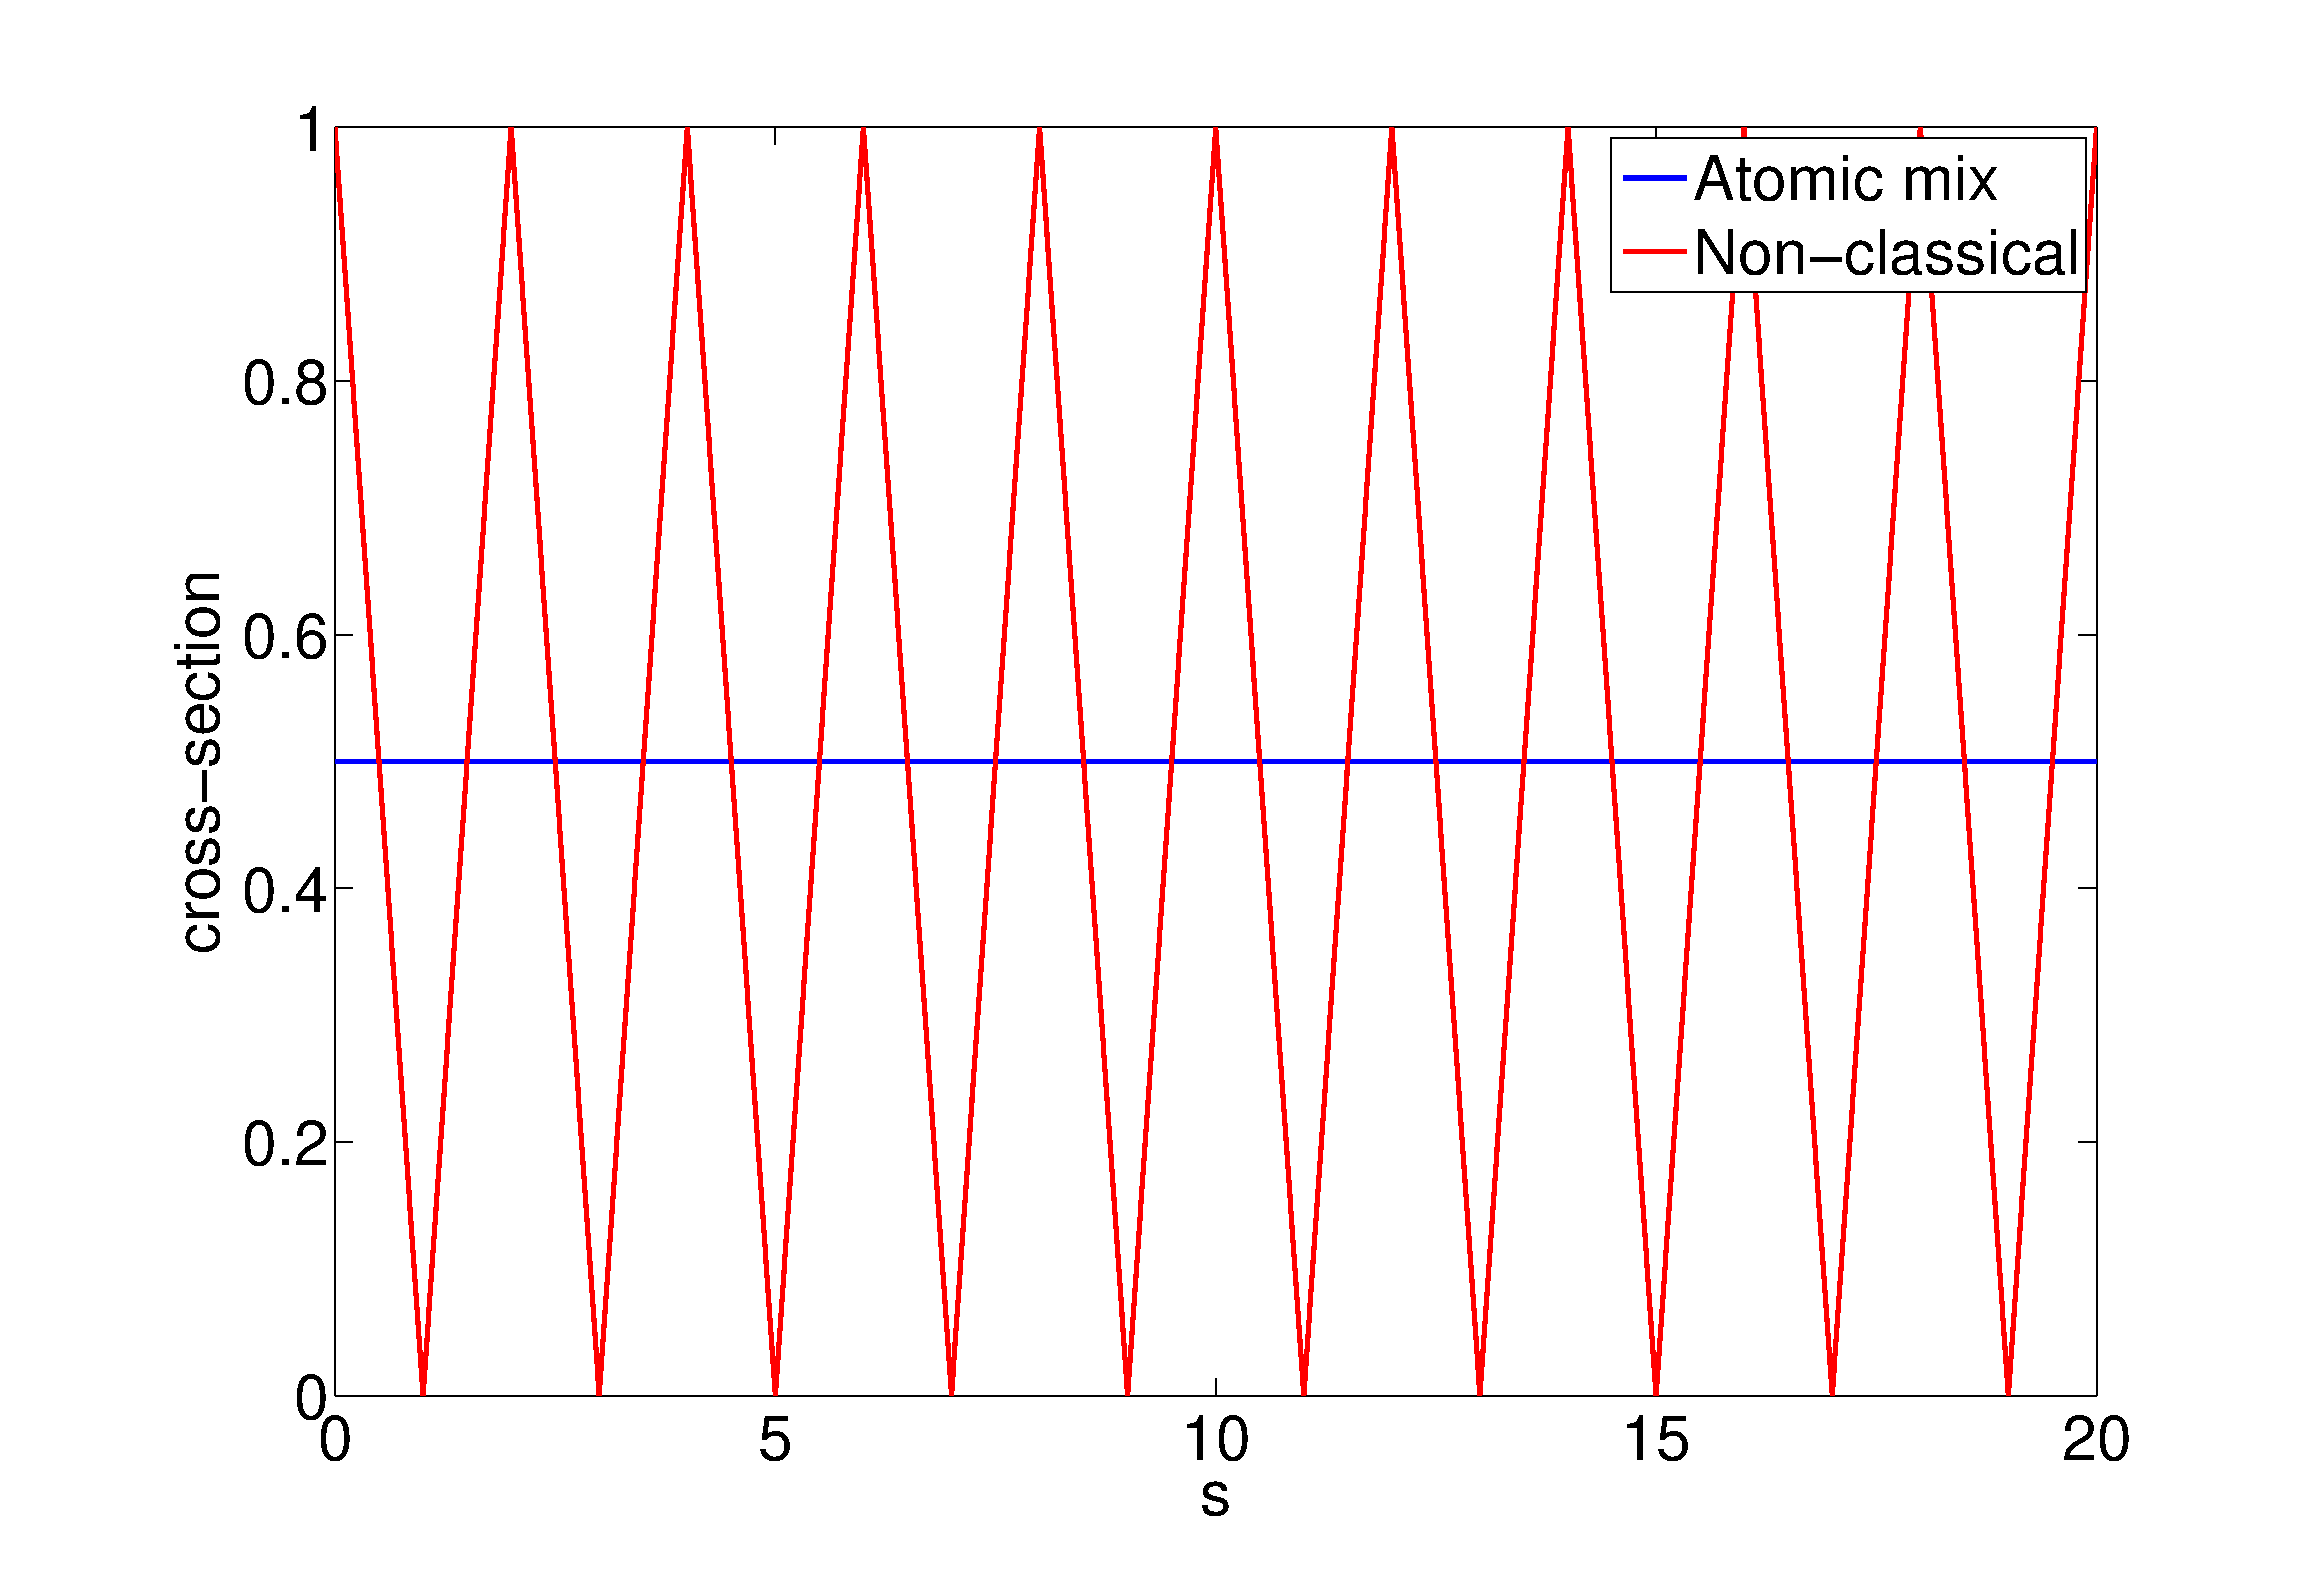
\includegraphics[scale=0.3]{fig6.pdf}
  \caption{$\bl \Sigma_t\bg$ and $\Sigma_t(s)$ for Problem Set {\bf B}}
  \label{fig6}
\end{figure}

For the numerical solution of this system, we can interpret the path-length $s$ as a pseudo-time variable.
We then solve \cref{eq20} using a finite volume method with explicit pseudo-time discretization according to \cite{hll83}.
Specifically, we adapt the scheme introduced in \cite{kry13} for moment models of the nonclassical transport equation.

This method is of first order in the pseudo-time variable $s$ and in the spatial variable $x$.
We choose a uniform grid $(x_m,s^n)$, where $x_{m+1} = x_{m} + \Delta x$ for all $m\in\mathbb{Z}$, and $s^{n+1} = s^n + \Delta s$ for all $n\in\mathbb{N}_0$.
Furthermore, we define $\psi_{m}^{n,\pm}= \psi^\pm(x_{m},s^n)$, $Q_m = \bl Q\bg (x_m)$, and $\Sigma_t^n=\Sigma_t(s^n)$.
The fully discretized system reads
\begin{subequations}\label[pluraleq]{eq21}
\begin{align}
	& \frac{\psi^{n+1,\pm}_m-\psi^{n,\pm}_m}{\Delta s} \pm \frac{\psi^{n,\pm}_{m+1}-\psi_{m-1}^{n,\pm}}{2\Delta x} - 
			\frac{\psi^{n,\pm}_{m+1}-2\psi_m^{n,\pm}+\psi_{m-1}^{n,\pm}}{2\Delta x}   + \Sigma_t^n \psi^{n,\pm}_m = 0, \label{eq21a}\\
	&  \psi_m^{0,\pm} = \frac{c}{2}\sum\limits_{n=0}^\infty \omega_n \Sigma_t^n\left( \psi_m^{n,+} + \psi^{n,-}_m\right)  +  \frac{Q_m}{2},\label{eq21b}	
\end{align}
\end{subequations}
% Maybe this is clear and I missed it, but (for my own knowledge), why is the partial derivative
% in s approximated differently than that in x? Is it because we are assuming the particles have
% a different behavior in s and x? Can you at some point go through with me why it is this way?
for some infinite quadrature rule given by the weights $\omega_n$.
The second order central differences arise as a numerical diffusion term, which is typical for HLL finite volume schemes.
\begin{figure}[htb]
  \centering
  \includegraphics[scale=1]{fig7.eps}
  \caption{Nonclassical scalar flux for Problem Set {\bf B} with $c_1=0.5$}
  \label{fig7}
\end{figure}

In our calculations, we cut off the integration at $s_{\text{max}}=4X=40$, and use the trapezoidal rule.
We use the same mesh interval $\triangle x=2^{-7}$ as for the previous models, and a CFL number $0.5$ (that is, $\triangle s = 2^{-8}$). 
Because of the coupling of the initial value to the full solution in \cref{eq20}, this system is solved in a source-iteration manner, where we iterate between \cref{eq21a,eq21b}.
Finally, the ensemble-averaged {\em nonclassical} scalar flux is given by $\bl\Phi_{NC}\bg(x) = \int_0^{40}[\psi^+(x,s)+\psi^-(x,s)]ds$. An example is depicted in \cref{fig7}.


\section{???}


Abstract

End of Introduction

Moments of $p(s)$

Diffusion Analysis

"Standard" Numerical results

Numerical results away from atomic mix limit

Conclusion

\pagebreak
\begin{singlespace}
\bibliography{references}
\bibliographystyle{ans}
\end{singlespace}

\end{document}
